\section{Klassifizierungsgenauigkeit der Anomalien}
\label{sec:eval_anomalieerkennung}
Bei der Anomalieerkennung werden Entscheidungswälder und FFNNs mit den besten ML-Modellen zur Standorterkennung trainiert und mit den drei Baseline-Modellen verglichen.
Tabelle \ref{tab:anomaly_detection_prediction_accuracy} zeigt die Klassifizierungsgenauigkeiten über die verschiedenen Standortkomplexitäten,
wobei die Klassifizierungsgenauigkeit $P(A)$ nochmal genauer in den Anteil der korrekten Klassifizierungen aufgeschlüsselt ist, wenn eine bzw. keine Anomalie vorlag.
Die trainierten FFNNs geben stets aus, dass keine Anomalie vorliegt.
Es ist unklar, warum die FFNNs sich so verhalten.
\begin{table}[h!]
    \hspace{-1cm}
    \begin{tabular}{ | l | c | c | c | c | c | c | c | c | }
        \hline
        Standorte & 9 & 16 & 17 & 25 & 32 & 48 & 52 & 102 \\\hline
        \multicolumn{9}{ | l |}{$P(A)$}\\\hline
        Entscheidungswald & 82,59\% & 81,19\% & 87,14\% & 84,91\% & 79,06\% & 83,47\% & 81,93\% & 76,00\% \\\hline
        FFNN & 77,88\% & 77,88\% & 77,88\% & 77,88\% & 77,88\% & 77,88\% & 77,88\% & 77,88\% \\\hline
        Topologie (DT) & 84,77\% & 30,57\% & 83,51\% & 79,76\% & 28,63\% & 24,97\% & 80,55\% & 29,47\% \\\hline
        Topologie (KNN) & 86,10\% & 52,17\% & 77,72\% & 79,30\% & 45,06\% & 41,92\% & 74,77\% & 43,55\% \\\hline
        \multicolumn{9}{ | l |}{Anteil korrekt klassifiziert, indem Anomalie vorlag}\\\hline
        Entscheidungswald & 34,86\% & 35,52\% & 52,58\% & 50,92\% & 32,21\% & 50,64\% & 23,21\% & 1,92\% \\\hline
        FFNN & 0,00\% & 0,00\% & 0,00\% & 0,00\% & 0,00\% & 0,00\% & 0,00\% & 0,00\% \\\hline
        \multicolumn{9}{ | l |}{Anteil korrekt klassifiziert, indem keine Anomalie vorlag}\\\hline
        Entscheidungswald & 96,14\% & 94,41\% & 97,05\% & 95,83\% & 92,48\% & 93,13\% & 98,96\% & 97,18\% \\\hline
        FFNN & 100,00\% & 100,00\% & 100,00\% & 100,00\% & 100,00\% & 100,00\% & 100,00\% & 100,00\% \\\hline
    \end{tabular}
    \caption{$P(A)$ über Standorte und Modelle zur Anomalieerkennung.}
    \label{tab:anomaly_detection_prediction_accuracy}
\end{table}
\newpage
Die Entscheidungswälder hingegen eignen sich besser für den Anomalieerkennungszweck.
Es werden zwischen 1,92\% und 52,58\% der Anomalien erkannt und zwischen 1,04\% und 7,52\% falsch als Anomalien erkannt.
Die Klassifizierungsgenauigkeit des Entscheidungswaldes zur Anomalieerkennung ist abhängig von der Klassifizierungsgenauigkeit zur Standorterkennung
und von der Standortkomplexität.
Je besser das Standorterkennungsmodell und je höher die Standortkomplexität, desto höher ist die Anomalieerkennungsrate.
Aus diesem Grund ist die Klassifizierungsgenauigkeit bei den Standortkomplexitäten, die mit dem Kodierungsansatz, der Kanten und Knoten kodiert, zusammenhängen,
geringer, als bei dem Kodierungsansatz, der nur die Knoten kodiert.
\newline
\newline
Abbildung \ref{fig:true_vs_predicted_anomaly} zeigt einen Ausschnitt der Anomalietestmenge, worauf der Entscheidungswald der Standortkomplexität 17 angewendet wurde.
Die Anomalie wird nicht kontinuierlich erkannt und es werden auch fälschlicherweise Standorte als Anomalien klassifiziert.
Allerdings treten falsch-positive Ergebnisse nur vereinzelt auf, wohingegen bei einer Anomalie, sehr häufig eine Anomalie erkannt wird.
Die falsch-positiven Ergebnisse können somit durch Ausnutzen dieser Fluktuationen vermieden werden,
indem beispielweise ein Schwellenwert an Ausschlägen in einer bestimmten Zeit eingeführt wird.
\begin{figure}[h!]
    \centering
    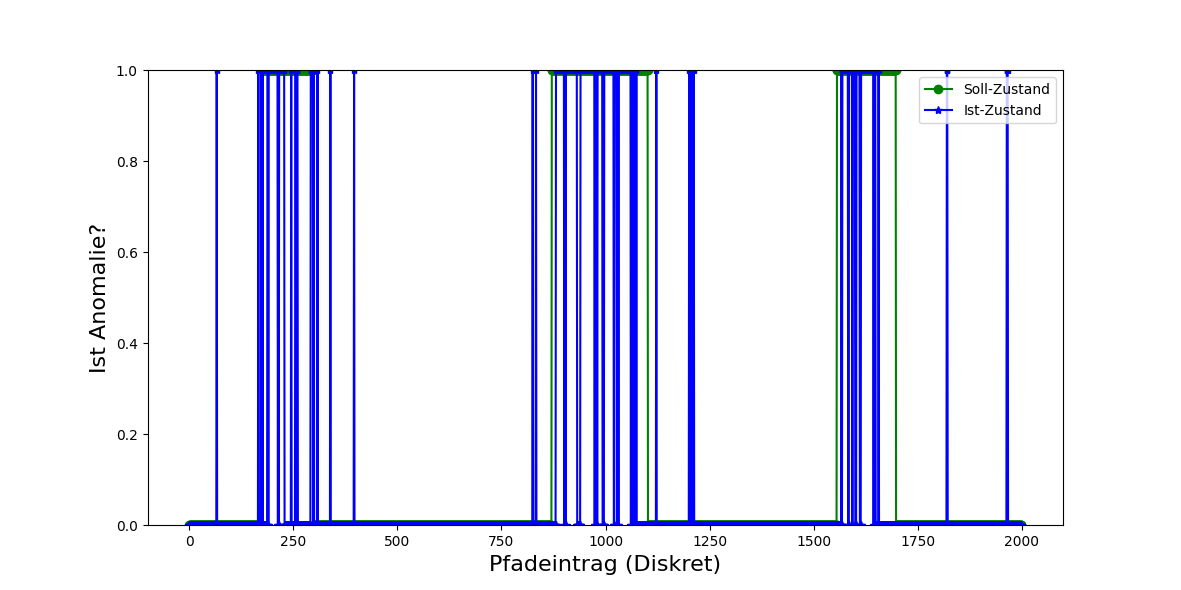
\includegraphics[width=\linewidth]{images/anomaly_true_vs_predicted.png}
    \caption{Ausschnitt der Klassifizierungsergebnisse auf der Anomalietestmenge mit dem Entscheidungswald der Standortkomplexität 17. }
    \label{fig:true_vs_predicted_anomaly}
\end{figure}